\documentclass[10pt,twocolumn]{article}

\usepackage{fixltx2e}
\usepackage{cuted}
\usepackage{titling}
\usepackage[T1]{fontenc}
\usepackage{lmodern}
\usepackage{graphicx}
% \graphicspath{ {./images/} }

\begin{document}

\setlength{\droptitle}{-4em}     % Eliminate the default title vertical space
\addtolength{\droptitle}{-20pt}   % Used for title adjustment

\title{%\vspace{-40cm}
Instituto Superior Técnico \\
\huge Highly Dependable Systems Project - Stage 1 \\
\huge Dependable Public Announcement Server
}

\author{Iulian Puscasu, 87665}

\date{April 7, 2020}

\maketitle

\section{Introduction }
The goal of the project is to design and implement a Dependable Public Announcement Server (DPAS) where public information and facts can be posted, tracked and verified.
The implemented project uses grpc for client-server communication and hybrid encryption for message transmission.

\section{Design}

\subsection{Database design}

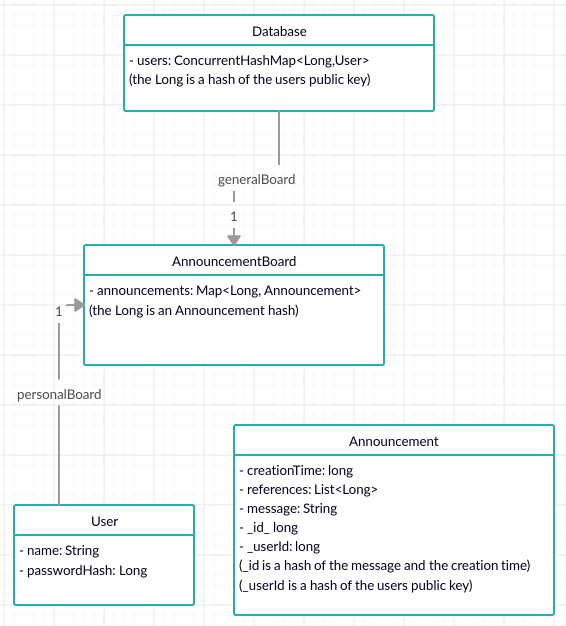
\includegraphics[scale=0.375]{database-domain}

\subsection{Available functions}

The postGeneral and readGeneral functions are missing only because of lack of time.
Everything needed for them to work is already implemented in protobuf and the domain.

To register and make posts, a user must provide a password. A hash will be saved in the server and this provides us with 2 factor authentication.

\subsection{Message design}

Firstly, every message is sent through a grpc channel, which has built in serialization.
This makes it harder for an attacker to read the data if he doesn't know the message structure.

Secondly, the messages sent to the server are encrypted using a random generated 128 bit AES key and a 1024 bit RSA keypair.
(These keys could be larger for added security)

The messages going from the server to the clients aren't encrypted since they hold no relevant data.

The encryption is as follows:

$(data + signature(data)_{client\_priv\_key})_{aes\_key} + aes\_key_{server\_pub\_key} + pub\_key$

First, we create a signature of our request data using the clients private key.

At the same time, we generate a random AES key. This functions as a nonce and also allows us to use a more parallelizable ECB Cipher mode.

Then we put the data and the signature together and encrypt them using the AES key.

Afterwards, we encrypt the AES key using the servers public RSA key.

What we send to the server are the previous two items plus the clients public key.

\section{Threat analysis and Protection Mechanisms}

In short, we get:

\begin{itemize}
    \item confidentiality from the server public key
    \item integrity and authentication from the Signature
    \item freshness from te AES key as it's used as a nonce. Plus every request contains a timestamp.
\end{itemize}

\subsection{Data confidentiality}

\subsubsection*{Possible Attacks}

Sniffing = Eavesdropping = Interception

\subsubsection*{Countermeasures}

The client public key is visible but only the server can decrypt the contents of the actual data in the request.

\subsection{Data integrity}

\subsubsection*{Possible Attacks}

Unauthorized data modification

\subsubsection*{Countermeasures}

The signature made from the data tells the server if the received request has been modified.
If we wanted we could make a log of the infraction, notify the actual user, send a fake response to the attacker, etc.

\subsection{Entity/Data-origin authentication (+ freshness)}

\subsubsection*{Possible Attacks}

Spoofing (man-in-the-middle or impersonation)

Replay attack

Replay to sender attack

Surreptitious forwarding

Message stealing

\subsubsection*{Countermeasures}

Spoofing is impossible without the servers private RSA key.

Replay attacks are detected with the RSA key, which functions as a nonce, in combination with a timestamp in every request.
The timesstamp is also verified with a signature and encrypted on top of that.

Message forwardind is fine, since there are no consequences if that happens. Only the server can read the message.
Message stealing cannot happen by anyone other than the server, but we trust the server at this stage.
If we wanted to prevent that, we could just add the source and destination of the request along with it.

\subsection{Data/service availability}

\subsubsection*{Possible Attacks}

DoS attack

\subsubsection*{Countermeasures}

Since this is only a single server, this is a weakness of this system.
Even then, thera are some attempts to improve concurrency:
\begin{itemize}
    \item gRPC internally creates a threadpool to handle RPCs
    \item The server handler is non-blocking
    \item The client stubs we use are Blocking but could be upgraded to listenable futures if client performance was desirable
\end{itemize}

\section{Other Dependability Guarantees}

The database only uses concurrent HashMaps, to support concurrency.

\end{document}
